\documentclass[a4paper,DIV=12,english]{scrartcl}
\usepackage[utf8]{inputenc}
\usepackage{fancyhdr}
\usepackage{bookmark}
\usepackage{graphicx}
\usepackage{hyperref}
\usepackage{xurl}
\usepackage[sorting=none, style=numeric-comp]{biblatex}
\addbibresource{ref.bib}
\usepackage{csquotes}
\usepackage[dvipsnames]{xcolor}
\usepackage[num]{isodate}
\usepackage{amsthm}
\usepackage{amssymb}
\usepackage{bbm}
\usepackage{amsmath}
\usepackage{tikz}
%\usepackage{pgfplots}
    %\usepgfplotslibrary{fillbetween}
\usepackage{svg}
\usepackage{braket}
\usepackage{caption}
\usepackage{subcaption}
\usepackage{placeins}
%\setlength\parindent{0pt}
\usepackage{wrapfig}
\usepackage{float}

% Fakesection
\newcommand{\fakesection}[1]{%
    \par\refstepcounter{section}                                        % Increase section counter
    \sectionmark{#1}                                                    % Add section mark (header)
    \addcontentsline{toc}{section}{\protect\numberline{\thesection}#1}  % Add section to ToC
    % Add more content here, if needed.
} 

\renewcommand{\footrulewidth}{0.5pt}
\pagestyle{fancy}
\fancyhf{}
\fancyhead[L]{\leftmark}
\fancyhead[R]{}

\fancyfoot[C]{Computational Physics: Explaining the Periodic Table}
\fancyfoot[R]{\thepage}

\title{Computational Physics: Explaining the Periodic Table}
\author{Stockholm University, Spring Term 2024 \\Max Maschke}
\date{May 14 2024}


\begin{document}
\maketitle


\tableofcontents
\newpage


\newpage
\section{Introduction}The aim of this project is to implement a self-consistent mean field algorithm to approximate the ground state electron density of atoms and their ionisation energies. It is part of the coursework for the computational physics class held at Stockholm University in 2024.

\section{Atomic Physics and Aspects of Density Functional Theory}
From a theoretical point of view, an atom is a quantum mechanical system in which electrons are bound by a central nuclear charge which is often approximated as a point charge of magnitude $Ze$. Despite their abundance and the limited number of particles involved, the fermionic nature of electrons is a major hindrance to the treatment of the electronic structure of atoms. As the wave function of a system with $N_e$ electrons is a function of $3N_e$ variables (neglecting the spin degree of freedom), the memory required to represent it on a grid with $m$ points per dimension scales rather unpleasantly as $m^{3N_e}$. For a conservative number of $m=100$ and $N_e=6$ electrons for, e.g., Carbon, $100^{18}=10^{36}$ numbers would have to be stored, which by far overwhelms the collective storage capacity of all computers on Earth. % TODO citation!

Luckily, the full wave function is not actually needed. According to a theorem due to Hohenberg and Kohn~\cite{kohn_hohenberg}, the ground state wave function is a unique functional of the ground state electron density, which is only a function of 3 variables, and vice versa. That is, in principle, all information that can be extracted from the wave function $\psi(\textbf{r}_1,\sigma_1, \dots, \textbf{r}_{N_e},\sigma_{N_e})$ can also be extracted from the density
\begin{equation}
    n(\textbf{r}) = N_e \sum_{\sigma_i}\int_{\mathbb{R}^3} \text{d}^{3(N_e-1)}\textbf{x}\,\left|\psi(\textbf{r},\sigma_1,\textbf{x}_2,\sigma_2,\dots,\textbf{x}_{N_e},\sigma_{N_e})\right|^2.
\end{equation}
This is the motivation behind density functional theory (DFT), which today is arguably the most important computational method in quantum chemistry. In this report, we explore a simple version of this approach that relies on finding a self-consistent radially symmetric single particle potential $V_\text{int}(r)$ such that the Slater-determinant
\begin{equation}
    \psi(\textbf{r}_1, \dots, \textbf{r}_{N_e}) = \frac{1}{\sqrt{N_e!}}\det 
    \begin{bmatrix}
\varphi_1(\textbf{r}_1) &\dots &\varphi_{N_e}(\textbf{r}_{1}) \\
\vdots & \ddots & \vdots \\
\varphi_{N_e}(\textbf{r}_{N_e}) &\dots &\varphi_{N_e}(\textbf{r}_{N_e}) 
    \end{bmatrix}
\end{equation} 
associated with the single-particle Hamiltonian (in atomic units)
\begin{equation}\label{eq:seq}
    \mathcal{H} = -\frac{1}{2}\partial_\textbf{r}^2 - \frac{Z}{r} + V_\text{int}(r)
\end{equation}
approximates the spatial component of the ground state of the full $N_e$-particle Hamiltonian. The ansatz for $V_\text{int}(r)$ includes two terms. The first is the direct electrostatic potential due to the charge density of the electrons. It must be obtained by solving Poisson's equation
\begin{equation}
    \partial_\textbf{r}^2 V_\text{int}^{\text{dir}}({r})= -4\pi n({r}) = -4\pi \sum_{i=1}^{N_e} \left|\varphi_i({r})\right|^2,
\end{equation}
for which the methods developed in the second-to-last hand-in can be employed due to the radial symmetry. The second term is an approximation to the exchange interaction or Pauli repulsion. It is derived for an ideal electron gas and reads
\begin{equation}
    V_\text{int}^{ex}({r}) = -3\left( \frac{3n({r})}{8\pi} \right)^{\frac{1}{3}}.
\end{equation}
Since $n(r)$ appears in both terms of $V_\text{int}(r) = V_\text{int}^{\text{dir}}({r}) + V_\text{int}^{ex}({r})$ but $n(r)$ requires knowledge of the solutions $\varphi_i(r)$ of $\mathcal{H}\varphi_i(\textbf{r}) = \varepsilon_i\varphi_i(\textbf{r})$, it is apparent that an iterative approach is needed. The most simple way to do this is to begin with $V_\text{int}(r) = 0$, calculate $n(r)$ and use this to solve the single particle Schrödinger equation again, until convergence. In practice, we check for convergence by observing if the total energy
\begin{equation}
        E_\text{tot} = \sum_{i\text{ occ.}} \left(\varepsilon_i - \frac{1}{8\pi}\int_{\mathbb{R}^3} \text{d}^3\textbf{r}\,\varphi_i(\textbf{r})^* V_\text{int}(r) \varphi_i(\textbf{r}) \right)
\end{equation}
settles up to a tolerance of $5\cdot 10^{-4}$. The ionisation energy of a neutral atom can simply be calculated by taking the difference of the total energy for the neutral atom and the total energy for a system with one electron less.

Due to the spherical symmetry of the problem, the single particle solutions can be decomposed as usual, i.e. $\varphi_i(\textbf{r}) = Y_{lm}(\theta, \phi)R_{nl}(r)$. This allows us to use the methods implemented last week.

The occupied single particle states in the atom are called orbitals and are labelled $n\,y^m$ where $n$ is the main quantum number, $y=s,p,d,f,\dots$ encodes $l=0,1,2,3,\dots$ and $m$ is the number of electrons in that orbital, which may not exceed $2(2l+1)$. For example, the lowest lying orbital is the $1s$-orbital which can accept at most 2 electrons.

In real atoms, the electrons do not exist in a Slater determinant but in a complex many particle state that is also influenced by Coulomb correlation, which is neglected here. Furthermore, the energy levels of the entire system are also affected by relativistic effects such as spin-orbit coupling, the finite size of the nucleus and, ultimately, QED effects like self-energy corrections.

\FloatBarrier
\section{Implementation and Numerics}
The algorithm sketched above is implemented as a \texttt{C++}-class \texttt{atom.h} that relies internally on the \texttt{b\_splines.h} class used by \texttt{collocation.h} and \texttt{spherical\_seq.h}, which are the collocation method boundary value problem solver and spherical single particle Schrödinger equation (SEQ) solver previously described in this course respectively. B-splines are thus used to represent both the wave functions and the interaction potential. The code can be found at~\cite{github} and it is also enclosed with this report.

As always when working with splines, the choice of knot sequence should reflect the nature of the problem to optimise numerical efficacy. While the radial functions live on an interval $[0, r_\text{max}]$, the \enquote{action} happens closer to the lower than to the upper bound, which is why it is prudent to increase the knot point density in that region. This is done in practice by choosing an exponential distribution of points
\begin{equation}
    r_0 = 0,\quad r_{i} = 10^{p_i}, \quad p_i = p_0 + i\Delta p, \quad \Delta p = \frac{\log r_\text{max} - p_0}{N-k-1}, \quad i = 1,\dots,N-k-1
\end{equation}
where $k=4$ is the order of the B-splines and $N$ is the number of points excluding ghost points appended at the interval bounds for technical reasons discussed in previous reports. We used $p_0 = -6$.

The main loop of the iteration can be summarised as follows:
\begin{enumerate}
    \item Solve SEQ with $V_\text{int}$
    \item Assign electrons to orbitals in ascending order of orbital energy
    \item Calculate electronic charge density 
    \item Check that $\int \text{d}r\, 4\pi r^2 n(r) = N_e$
    \item Solve Poisson's equation for $V_\text{int}$
    \item Calculate $E_\text{tot}$
    \item Check if $\Delta E_\text{tot} < \delta$ with $\delta = 5\cdot 10^{-4}$. If yes, end, if no, go to 1.
\end{enumerate}

To approve convergence and prevent oscillation of the total energy during the iteration, the interaction potential is interpolated between the last and current solution, i.e.
\begin{equation}
    V_\text{int}^{\text{mix}}(r) = (1-\eta)V_\text{int}^{\text{curr.}}(r) + \eta V_\text{int}^{\text{prev.}}(r),
\end{equation}
where $\eta=0.4$.

The approach described is applied to all elements from $Z=1$ to 108 and their first positive ions, using $r_\text{max}=10\,a_0$, 150 knot points for the SEQ solver and 300 points for the Poisson solver. 

Unfortunately, the method as implemented breaks down for heavier elements, which is surprising because the method should in theory perform better for larger systems. Phenomenologically, the iteration begins oscillating between different orbital configurations and thus no convergence is reached, resulting in large errors in the ionisation energy compared to experimental values from~\cite{NIST_ASD} as shown in figure~\ref{fig:ionergerr}. The heaviest atom treated with acceptable accuracy is element 55, Caesium.

Potential remedies which could not be tested due to time constraints include successively adding electrons during the iteration to allow the lower shells to settle, or including the second-to-last potential in the mixed interaction potential. Another possibility would be to manually prescribe which orbitals to fill, however, this would be rather inelegant.

For elements $Z<20$, though, the method works well within the constraints of the approximations made and errors are on the order of $10-20\%$.
\begin{figure}
    \centering
    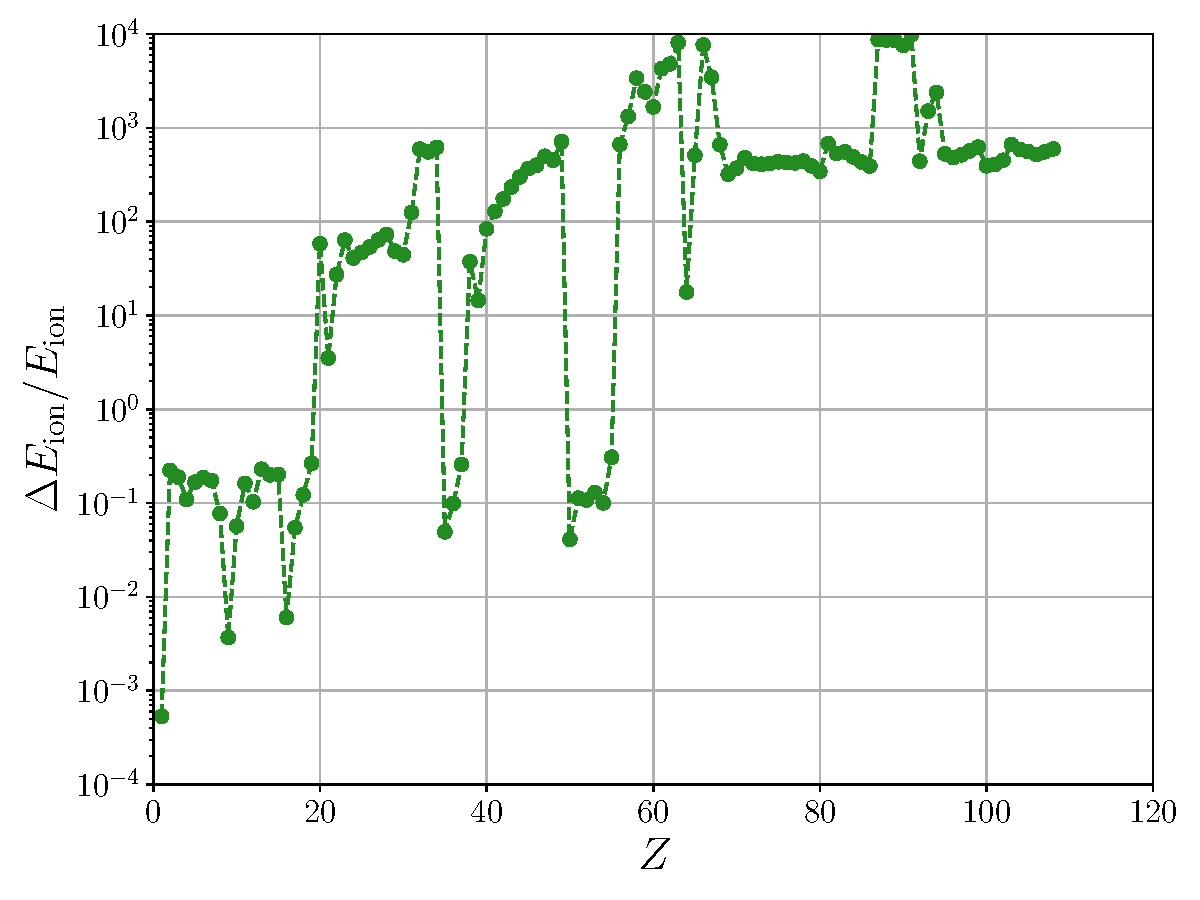
\includegraphics[width=0.65\textwidth]{../plots/ionerg_err.pdf}
    \caption{Relative error of the numerically obtained ionisation energy compared to experiment~\cite{NIST_ASD}. Elements with $Z<20$ show errors less than 20\%, while most heavier elements show comically large errors up to 4000\%, indicating that something went quite wrong.}
    \label{fig:ionergerr}
\end{figure}

\FloatBarrier
\section{Results}
The ionisation energies obtained are shown in figure~\ref{fig:ionerg}. While many elements with $Z\geq20$ have ionisation energies that are off by orders of magnitude, lighter ones generally follow the trend of the experimental data well, even though the numerical results do not fully capture all details of the true energy progression. For example, the model fail to predict that Oxygen has a lower ionisation energy than Nitrogen. Also, the model greatly underestimates the ionisation energy for Helium, which ought to have the highest ionisation energy of all elements, which the model assigns to Neon.

It can be seen that the noble gases (Helium, Neon, Argon, Krypton and Xenon) and the alkaline metals (Lithium, Sodium, Potassium, Rubidium and Caesium) seem to be well suited to be treated by the method because it works for them even after $Z=20$ up to Xenon and Caesium respectively when the algorithm has already broken down for the other elements. It is notably the transition metals which appear to be problematic.

For the light elements, we see that the noble gases are difficult to ionise while the alkaline metals are more \enquote{eager} to be rid of one of their electrons, which is in line with what we expect.

\begin{figure}
    \centering
    \begin{subfigure}{0.49\textwidth}
        \centering
        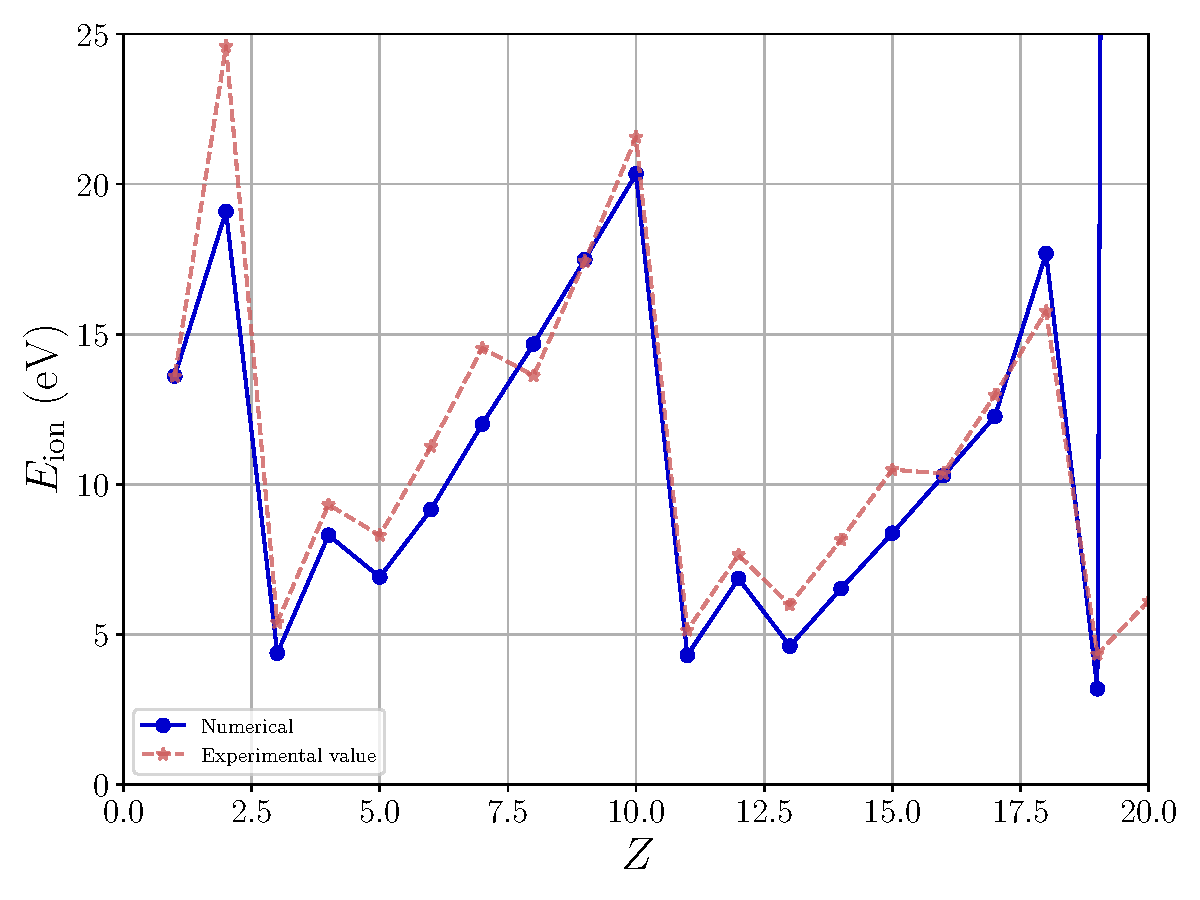
\includegraphics[width=\textwidth]{../plots/ionerg.pdf}
        \caption{$Z=1,\dots,19$}
        \label{subfig:ionerg_window}
    \end{subfigure}
    \begin{subfigure}{0.49\textwidth}
        \centering
        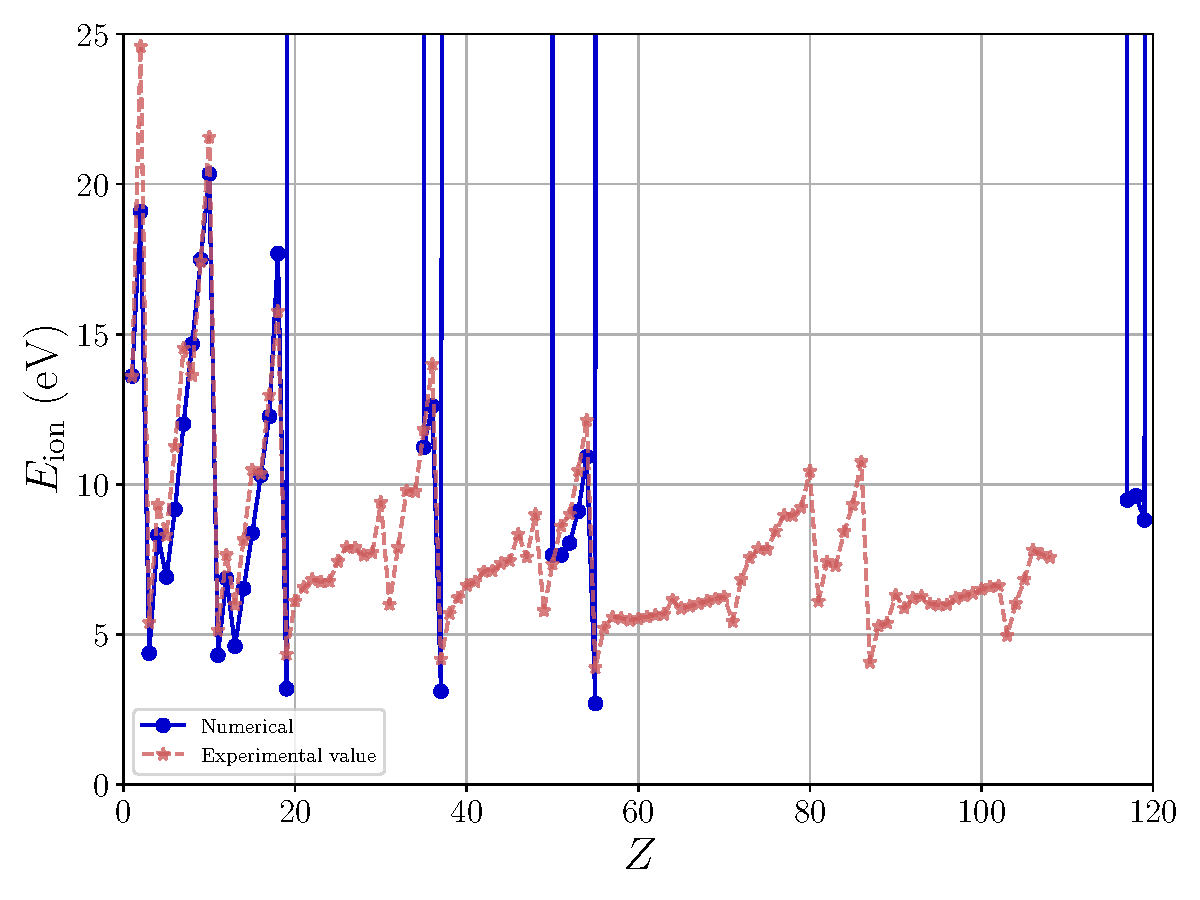
\includegraphics[width=\textwidth]{../plots/ionerg_full.pdf}
        \caption{Full range}
        \label{subfig:ionerg_full}
    \end{subfigure}
    \caption{Numerically obtained atomic ionisation energies for elements 1 to 19 \ref{subfig:ionerg_window} and full range \ref{sub@subfig:ionerg_full}. Many elements with $Z\geq20$ have ionisation energies that are off by orders of magnitude. Experimental values from~\cite{NIST_ASD}.}
    \label{fig:ionerg}
\end{figure}

The scaled electron densities $4\pi r^2 n(r)$ for a selection of atoms are shown in figure~\ref{fig:wfs}, where the scaling ensures that the curves integrate to $N_e$. The successive filling of orbitals can be observed and the reported orbital fillings are in agreement with literature.

\begin{figure}
    \centering
    \begin{subfigure}{0.49\textwidth}
        \centering
        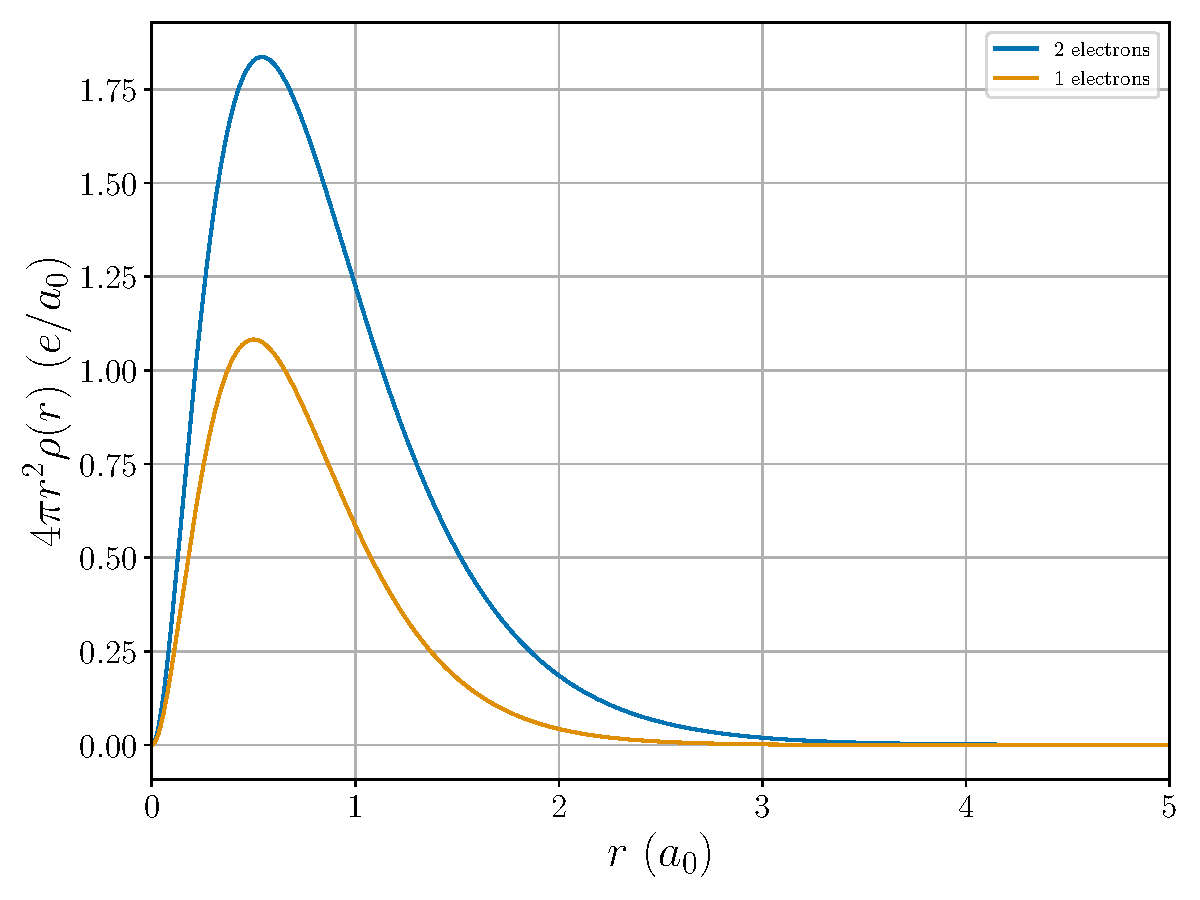
\includegraphics[width=\textwidth]{../plots/density/density_2.pdf}
        \caption{Helium ($Z=2$). \\$1s^2$ / $1s^1$.}
        \label{subfig:wf2}
    \end{subfigure}
    \begin{subfigure}{0.49\textwidth}
        \centering
        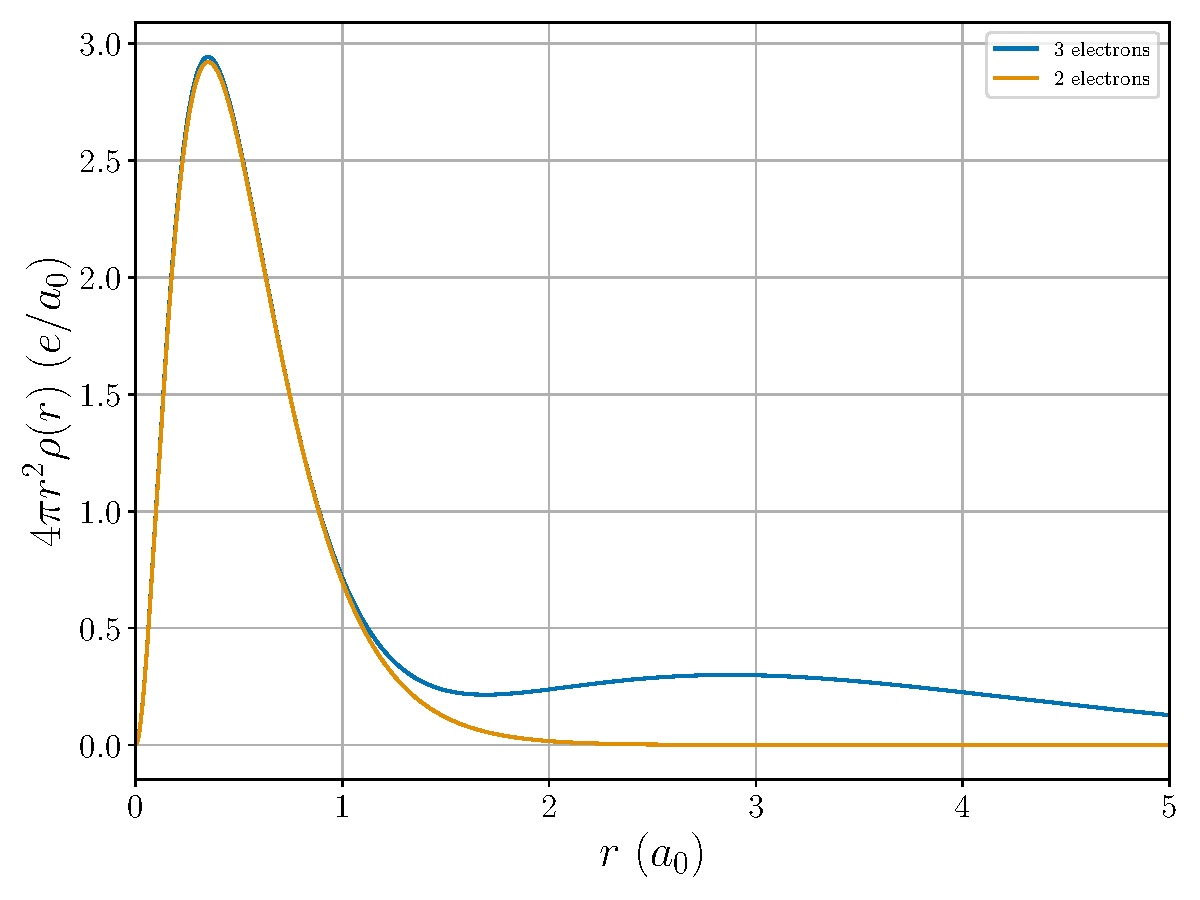
\includegraphics[width=\textwidth]{../plots/density/density_3.pdf}
        \caption{Lithium ($Z=3$). \\ \ [He]$2s^1$ / [He].}
        \label{subfig:wf3}
    \end{subfigure}
    \begin{subfigure}{0.49\textwidth}
        \centering
        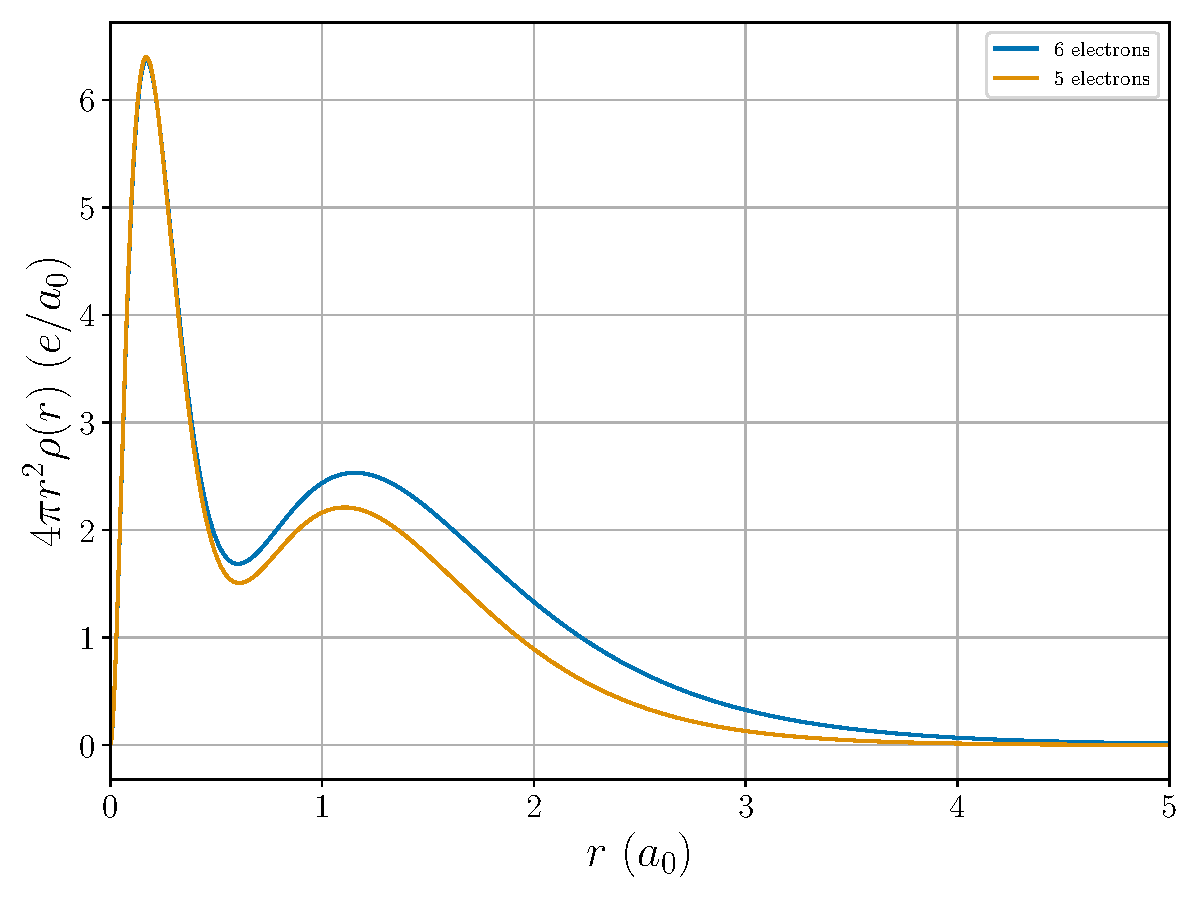
\includegraphics[width=\textwidth]{../plots/density/density_6.pdf}
        \caption{Carbon ($Z=6$). \\ \ [He]$2s^2 2p^2$ / [He]$2s^2 2p^1$.}
        \label{subfig:wf6}
    \end{subfigure}
    \begin{subfigure}{0.49\textwidth}
        \centering
        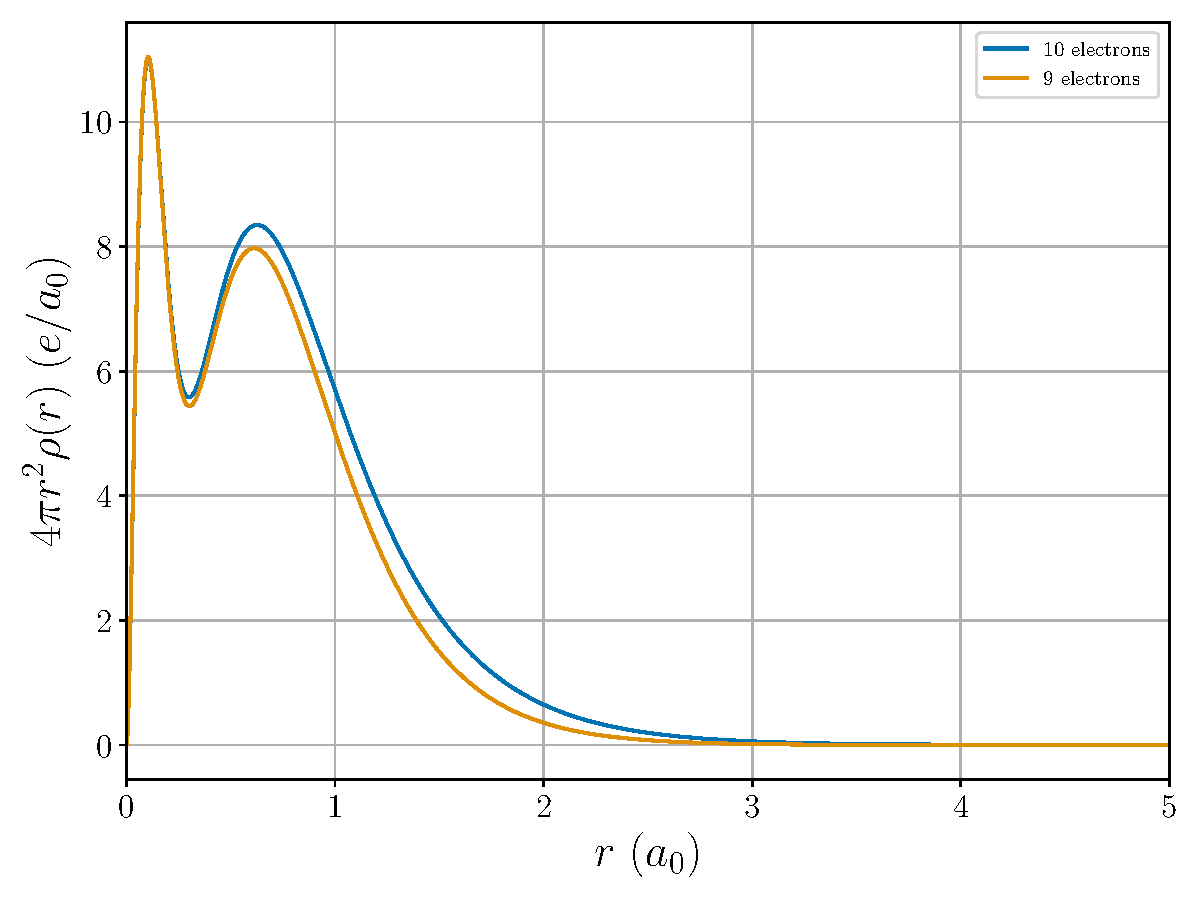
\includegraphics[width=\textwidth]{../plots/density/density_10.pdf}
        \caption{Neon ($Z=10$). \\ \ [Ne] / [He]$2s^2 2p^5$.}
        \label{subfig:wf10}
    \end{subfigure}
    \begin{subfigure}{0.49\textwidth}
        \centering
        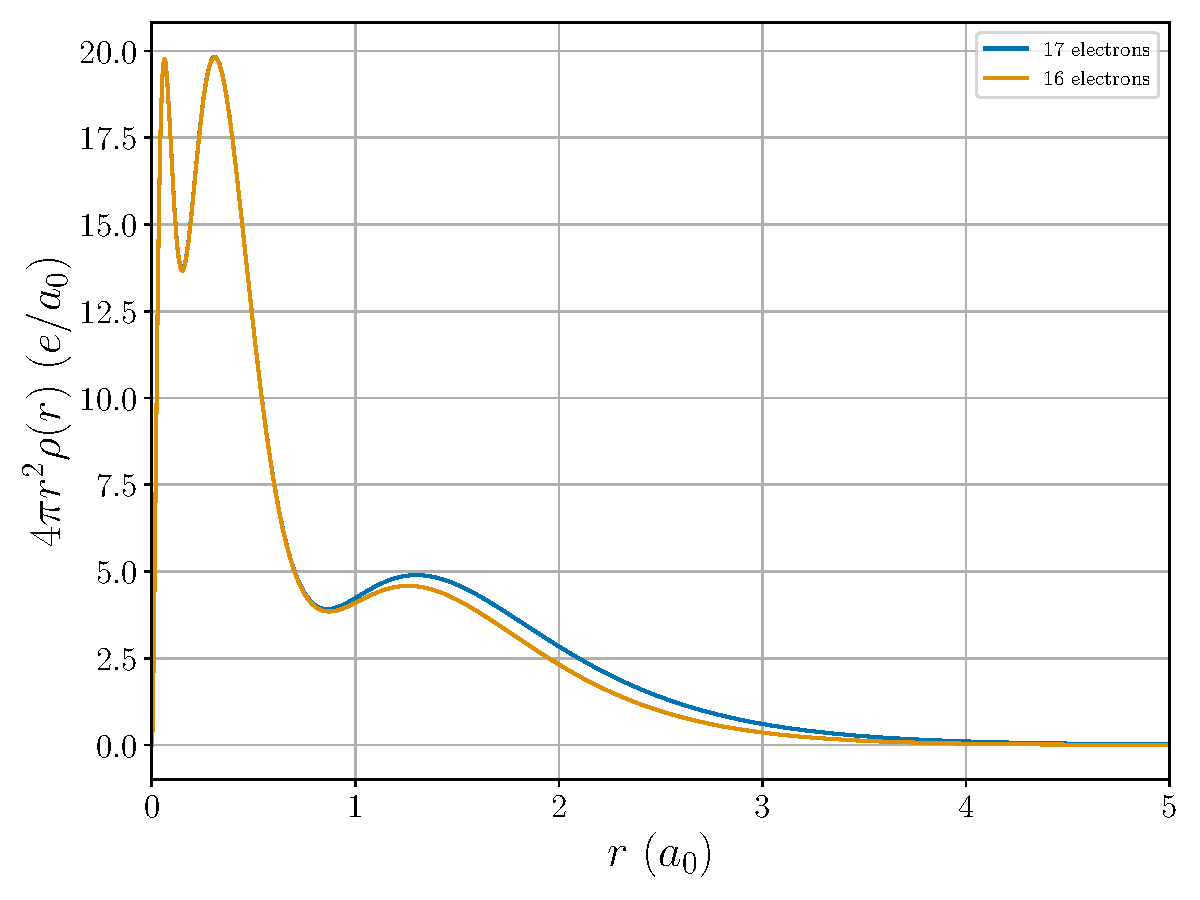
\includegraphics[width=\textwidth]{../plots/density/density_17.pdf}
        \caption{Chlorine ($Z=17$). \\ \ [Ne]$3s^2 3p^5$ / [Ne]$3s^2 3p^4$.}
        \label{subfig:wf17}
    \end{subfigure}
    \begin{subfigure}{0.49\textwidth}
        \centering
        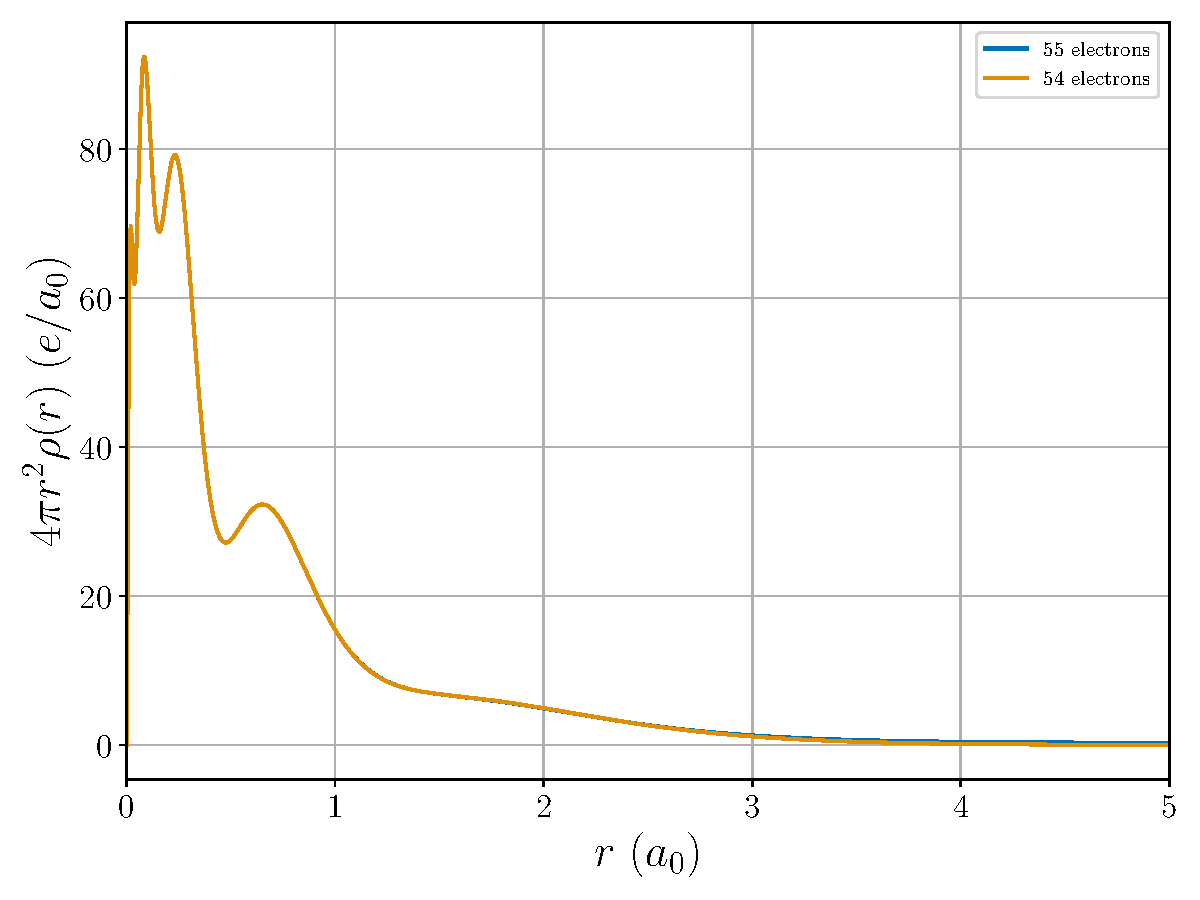
\includegraphics[width=\textwidth]{../plots/density/density_55.pdf}
        \caption{Caesium ($Z=55$). \\ \ [Xe]$6s^1 $ / [Xe]}
        \label{subfig:wf55}
    \end{subfigure}
    \caption{Scaled electron density $4\pi r^2 n(r)$ for a selection of atoms. The curves integrate to $N_e$. Successive filling of orbitals can be observed. Electronic structure of atom / ion.}
    \label{fig:wfs}
\end{figure}

Figure~\ref{fig:pots} shows the self-consistent interaction potentials for a selection of atoms. Light elements show a pronounced exchange cusp for small $r$. For heavy elements, the effect of exchange is minimal and the direct term dominates. The exchange potential seems to look increasingly delta-like for heavier elements.

\begin{figure}
    \centering
    \begin{subfigure}{0.49\textwidth}
        \centering
        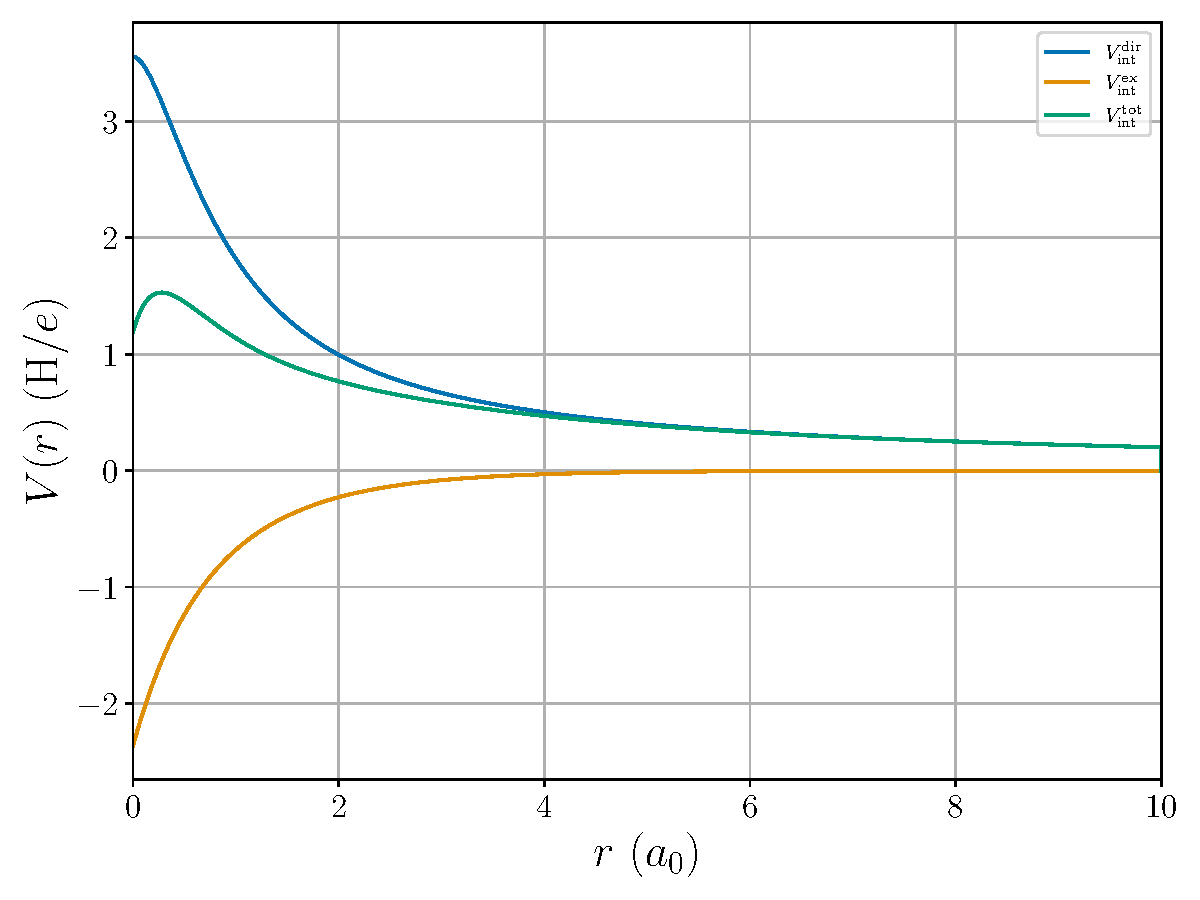
\includegraphics[width=\textwidth]{../plots/potentials/potential_2.pdf}
        \caption{Helium ($Z=2$)}
        \label{subfig:pot2}
    \end{subfigure}
    \begin{subfigure}{0.49\textwidth}
        \centering
        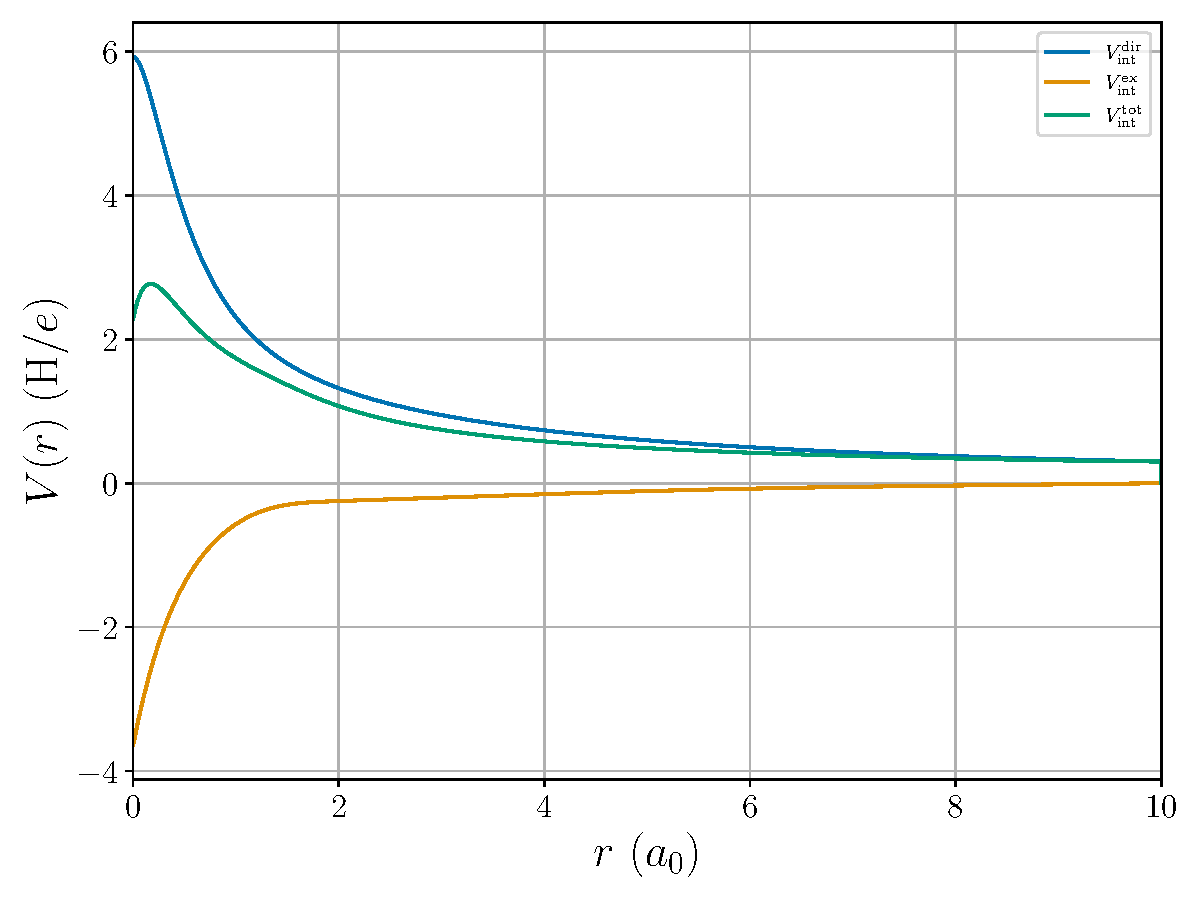
\includegraphics[width=\textwidth]{../plots/potentials/potential_3.pdf}
        \caption{Lithium ($Z=3$)}
        \label{subfig:pot3}
    \end{subfigure}
    \begin{subfigure}{0.49\textwidth}
        \centering
        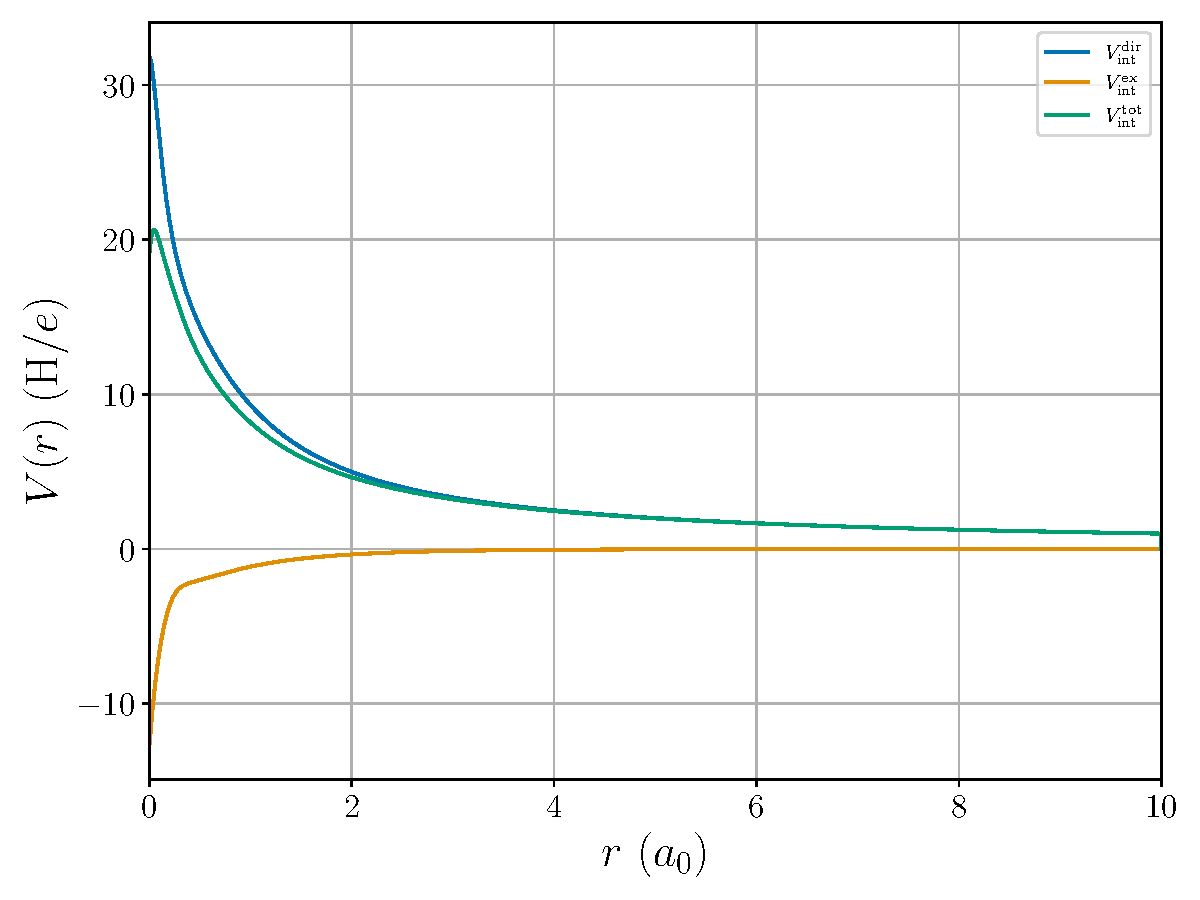
\includegraphics[width=\textwidth]{../plots/potentials/potential_10.pdf}
        \caption{Neon ($Z=10$)}
        \label{subfig:pot10}
    \end{subfigure}
    \begin{subfigure}{0.49\textwidth}
        \centering
        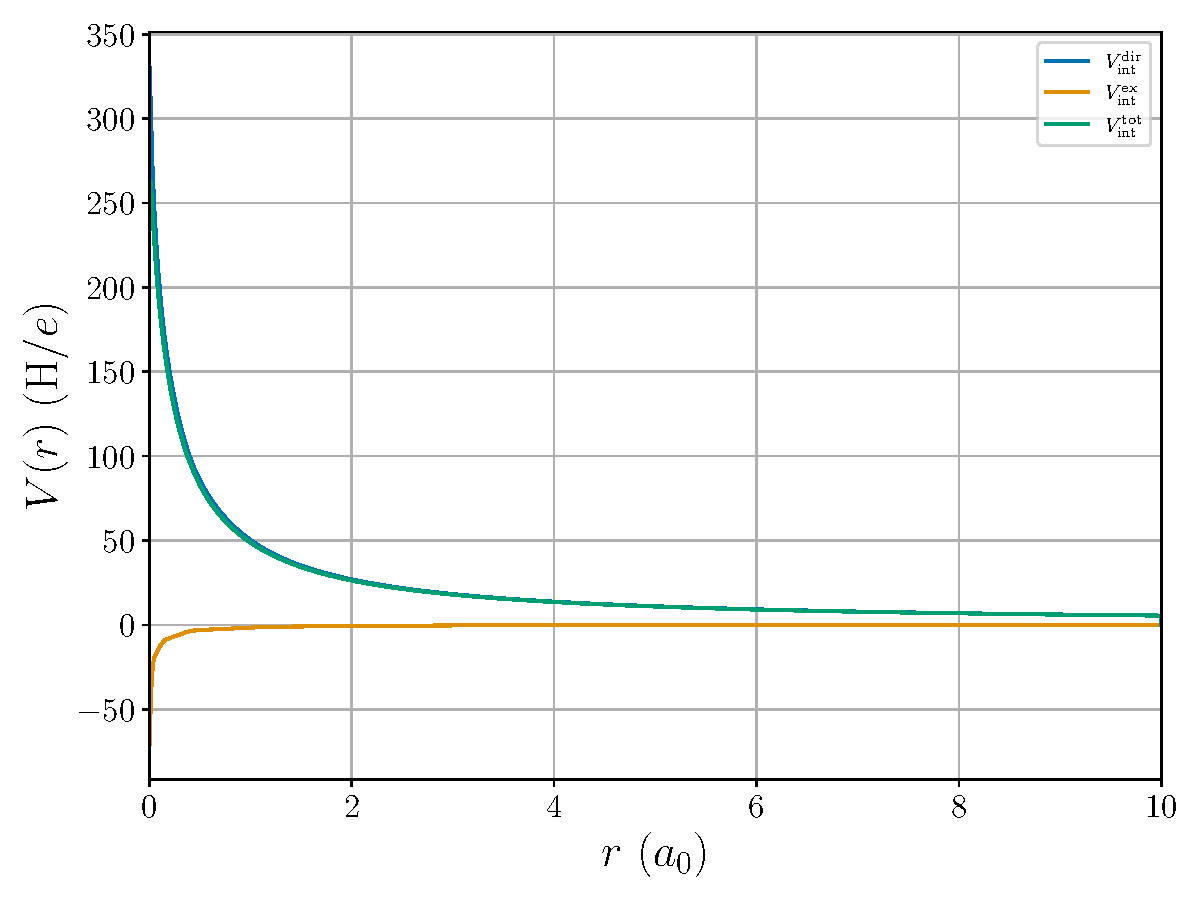
\includegraphics[width=\textwidth]{../plots/potentials/potential_55.pdf}
        \caption{Caesium ($Z=55$)}
        \label{subfig:pot55}
    \end{subfigure}
    \caption{Numerically obtained self-consistent electronic interaction potential. Light elements show a pronounced exchange cusp for small $r$. For heavy elements, the effect of exchange is minimal and the direct term dominates. The exchange potential seems to look increasingly delta-like for heavier elements.}
    \label{fig:pots}
\end{figure}

\FloatBarrier
\section{Conclusion}
The results obtained using the algorithm implemented are encouraging for light elements but problematic for heavy elements, which we sadly were not able to fix in time. However, we can observe some notable properties of the different groups of elements, especially noble gases and alkaline metals.

\FloatBarrier
\newpage
\fakesection{References}
\printbibliography


\end{document}
